\chapter{Further work on the model}
\label{secondPhaseOfModelingCyberInsurance} 

So far we have build a model reflecting how the purchase of cyber-insurance can force the formation of insured sub-graphs. As described earlier, the sub-graph would benefit from forming a star network. In this chapter our focus will be to show how we could force the sub graph to form a start topology. 

In the previous models our payoff equation has generated payoffs according to a nodes own earnings, in addition to the extra payoff, $\beta$, received when establishing a new connection. To be able to force the creation of a start topology, we need a new approach which allows nodes to increase their payoffs due to positive network externalities when connecting to the same node. Our idea is based on the paper from Jackson and Wolinsky \cite{jackson1996strategic} and a network formation game in \cite{jackson2005survey}. 

\section{The connection game}
The connection game reflects not only the benefit from establishing connections to other people, but also the benefits from indirect connections. Meaning, in addition to the benefit from the direct connection, a node will also benefit from "a friend of a friend", although the benefit will be a factor lower than the direct connection, also "friends of a friend of a friend" will generate benefit and so forth. The payoff will be calculated relative to the distance between different nodes.


\begin{figure}[h]
\centering
  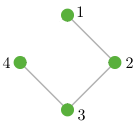
\includegraphics[width=0.2\linewidth]{../Figures/connectionGame.png}
  \caption{\label{fig:connectionGame} Four nodes interconnected with each other.}
\end{figure}For instance, node 1 in the following network depicted in figure \ref{fig:connectionGame}, will benefit $\beta$ from node 2, $\beta^{2}$ from node 3 and $\beta^{3}$ from node 4. The benefit will decrease relative to the shortest path between two nodes as long as $\beta < 1$. Hence the payoff a node receives from the network equals: 

\begin{equation}
\sum_{j\neq i}^{} \beta_{ij}^{d(ij)} - \sum_{j:ij\in g}^{} {I_{l}}_{ij}, 
\label{connecetionGame}
\end{equation}

where $d(ij)$ represents the shortest path between node $i $ and node $j $, and ${I_{l}}_{ij}$ represents node i's cost of insuring a link between the two nodes. To simplify the model we choose a symmetric connection process where $\beta$ and $I_{l}$ is set to a global value. 



TODO: 

To analyze the model we need to look at what efficiency is. 
How can we create a stable star topology

plot the different equations and discuss it. plot with real values from the model.

